\chapter{Proposed Work}\label{ch:Proposed}

\section{Task 1:}

\section{Task 2: Feture Ranking}

subsection{Performance evaluation}

The proposed FR metrics will be tested and compared according to the different combinations and methods in table\ref{tab: methods}. The features are removed one by one and classifiers are trained to observe the performance degradation. 
Preliminary results for \emph{ionosphere} dataset with Gaussian SVM is shown in fig. 

For this example dataset, we can observe that removing unnecessary features helps improve the classifier performance to some extent. Further, the proposed FR metrics outperform the existing method in identifying irrelevant features in the initial stage. These preliminary results show the potential of the proposed metrics and validate the need for further investigation. Similarly, performance will be analyzed for common, synthetic, and real-world datasets. 

% \begin{figure}[!t]
%     \centering
%     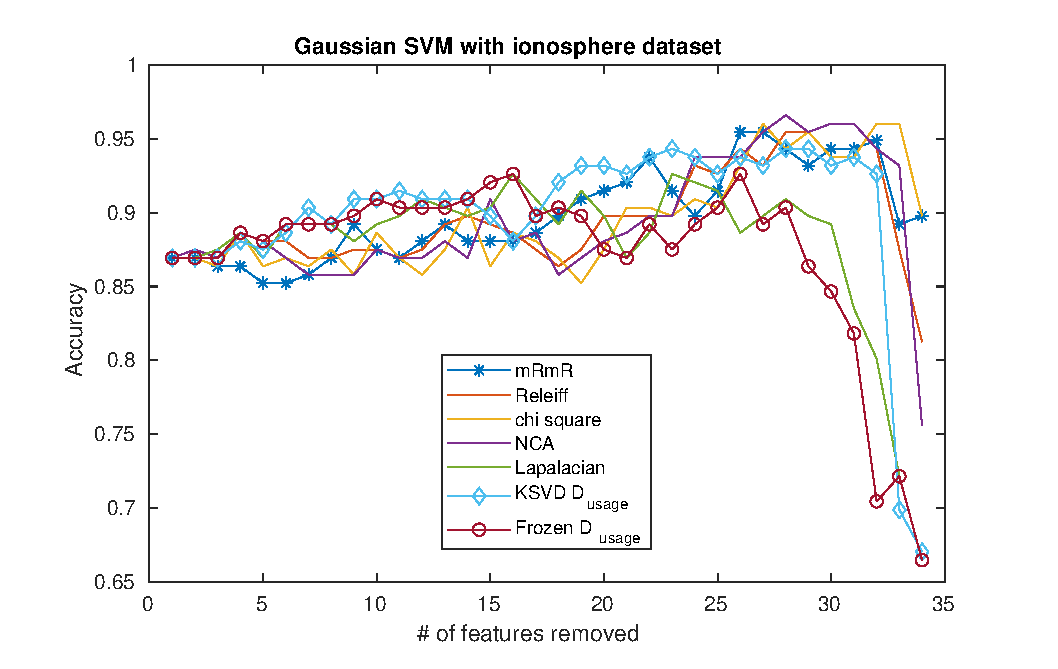
\includegraphics[width=\columnwidth]{figures/SR/ion_gauss.eps}
%     \caption[ionosphere]{Classifier performance degradation with number of features removed. It can be observed that the proposed methods have less performance degradation than the common FR metrics.}\label{fig: FR_degradation}
% \end{figure}

\begin{table}
\centering
\caption{Methods used in MATLAB environment}\label{tab: methods}
\begin{tabular}[!tbh]{*{3}{c}} 
\toprule
Dataset        & FR methods                        & Classifier method  \\ 
\toprule
Credit ratings & mRMR                              & Gaus SVM               \\ 
Ionosphere              & RELEIFF                           & Lin SVM            \\ 
letters              & $\chi^2$-test                     & Quad SVM           \\ 
               & NCA                               & Pol SVM                   \\
               &    $D_{map}$                          & Logistic regression \\
               &    $D_{util}$                        & Neural Network\\
\bottomrule
\end{tabular}
\end{table}

\subsection{tasks}
Following tasks will be completed for the achievement of the proposed goals and objectives

\begin{enumerate}
    \item Achieve similar performance degradation to existing FR methods within $95\%$ confidence interval within three months
    
    Some of the common FR methods will be considering are Releiff\cite{Kononenko1997}, mRMR\cite{Ding2005}, NCA\cite{Goldberger2005}, $\chi^2$-test, and PPCA\cite{Tipping1999}. These methods will be tested using common dataset such as, \textit{credit ratings}, \textit{ionosphere}, \textit{letters}, and synthetic data.    
    
    
    \begin{enumerate}
        \item Perform mathematical analysis of the proposed metrics with common FR metrics
        
        Each of the considered FR methods evaluates a different aspect of the features. We will discuss the theoretical similarities and differences of each metric compared to the proposed metrics.
        
        \item Perform the test with common FR methods and common data sets in one month
        
        The ranking given by different FR methods will be compared to the proposed metrics. The ranking given by common methods will be averaged and ranked. Then averaged ranking and proposed ranking will be compared to get a value of how many features matched the ranking.  Will discuss the experimental differences and similarities to understand the effect of data type and training hyper-parameters. Identify sensitiveness to the different data.
        
        \item Record performance degradation with feature removal and training times for each FR method
        
        The features are removed one by one by the ranking and the machine learning classifier performance will be measured. 
        
        \item Evaluate, compare, and improve the results in two months to $95\%$ confidence interval.
        
        The performance degradation will be compared to establish the shortcomings. Improvements to the metrics such as normalization and log-mapping can be introduced to improve performance.
        
    \end{enumerate}
    
    \item Improving the performance on imbalanced data by incorporating two other discriminatory SR methods in 4 months
    
    K-means singular value decomposition (KSVD)\cite{Aharon2006} is an efficient algorithm for SR-based methods. However, it is an unsupervised dictionary learning method and cannot incorporate label information. Hence, supervised dictionary learning algorithms will be tested with proposed metrics to improve the feature interpretability.
    
    \begin{enumerate}
    
        \item Finalizing the LCKSVD and Frozen KSVD data representation pipeline in two months.
        
        To incorporate class label information several variations of the KSVD algorithms exist. Two of the popular methods are label-consistent KSVD (LCKSVD)\cite{Jiang2011}, and Frozen KSVD\cite{Carroll2017}. The pipeline will be finalized so the class-wise FR can be generated with the proposed metrics. 
        
        \item Testing two other discriminatory SR methods and evaluating the performance to identify the best methods for the FR metric.
        
        Another two supervised dictionary learning methods are discriminatory KSVD (DKSVD)\cite{Zhang2010} and discriminative dictionary learning-based SR classification (DDL-SRC)\cite{Kong2021}. These methods will be included in the pipeline so that the researchers would have multiple choices to carry out FR metrics to interpret the data.
        
    \end{enumerate}
    
    \item Testing FR on Satellite images for classification for LULC tasks
    
    Satellite image classification is a challenging problem due to the high variability of the images, lack of reliable ground truth labels, and an abundant presence of atmospheric noise. Researchers use hand-crafted features and evaluate these images to identify land usage and land coverage. We will use the proposed FR metrics to identify and rank important/relevant features in different LULC scenarios. 
    
    \begin{enumerate}
        \item Training ML model with Sat-4, and Sat-6 dataset in three months
        
        Sat-4 and Sat-6\cite{Basu2015} are two widely used dataset for LULC tasks and has been benchmarked by various researchers\cite{Dundar2019, Pan2019, Li2018, Huang2017, Tang2014}. We will develop several ML models including SVM\cite{Vapnik1998}, logistic regression\cite{Wright1995}, and neural networks to train on the dataset.
        
        \item Evaluate the performance of models concerning other FR methods in five months
        
        The features will be removed according to rankings given by different FR methods, and Models will be re-trained with the remaining features. The performance degradation will be evaluated to assess the performance of the proposed metrics.
        
    \end{enumerate}
    \item Testing FR on Binary files to detect malware using control flow graphs (CFG)
    
    Detecting computer malware by just examining the binary files is challenging. Since, most of the vulnerabilities occur as run-time events, and depend on platform weaknesses; detecting malicious behavior is hard, without running them on targeted platforms. A common approach is to generate control flow graphs (CFG) to analyze graph structure\cite{}. Hence, we will be using the FR metric to identify the most important graph nodes and edges for the ML tasks.
    
    \begin{enumerate}
        \item Creating dataset of Benign and Malware dataset in two months
        
        A database with malware is provided by an anti-virus company \textit{Hoplite}\cite{}, and a database of benign programs has to be curated by scrapping the online app-stores\cite{}. These datasets will comprise different variations of malware and benign software.
        
        \item Incorporating SR methods into graph embedding learning in three months
        
        SR methods are not commonly used in graph analysis\cite{} pre-processing. Hence, a pipeline to incorporate the SR method has to be developed.
        
        \item Evaluate the performance of models concerning other FR methods in five months
        
        The graph nodes and edges will be removed according to rankings given by different FR methods, and the performance degradation will be evaluated to assess the performance of the proposed metrics.
        
    \end{enumerate}
\end{enumerate}
\section{Task 3:}

\section{Timeline}